\chapter{Background}
\label{chap:background}

% A more extensive coverage of what's required to understand your work.
% In general you should assume the reader has a good undergraduate
% degree in computer science, but is not necessarily an expert in the
% particular area you've been working on. Hence this chapter may need to
% summarize some ``text book'' material.
%
% This is not something you'd normally require in an academic paper, and
% it may not be appropriate for your particular circumstances. Indeed,
% in some cases it's possible to cover all of the ``background''
% material either in the introduction or at appropriate places in the
% rest of the dissertation.

%% The state of modern compiler development/usage

\begin{figure}[H]
    \centering
    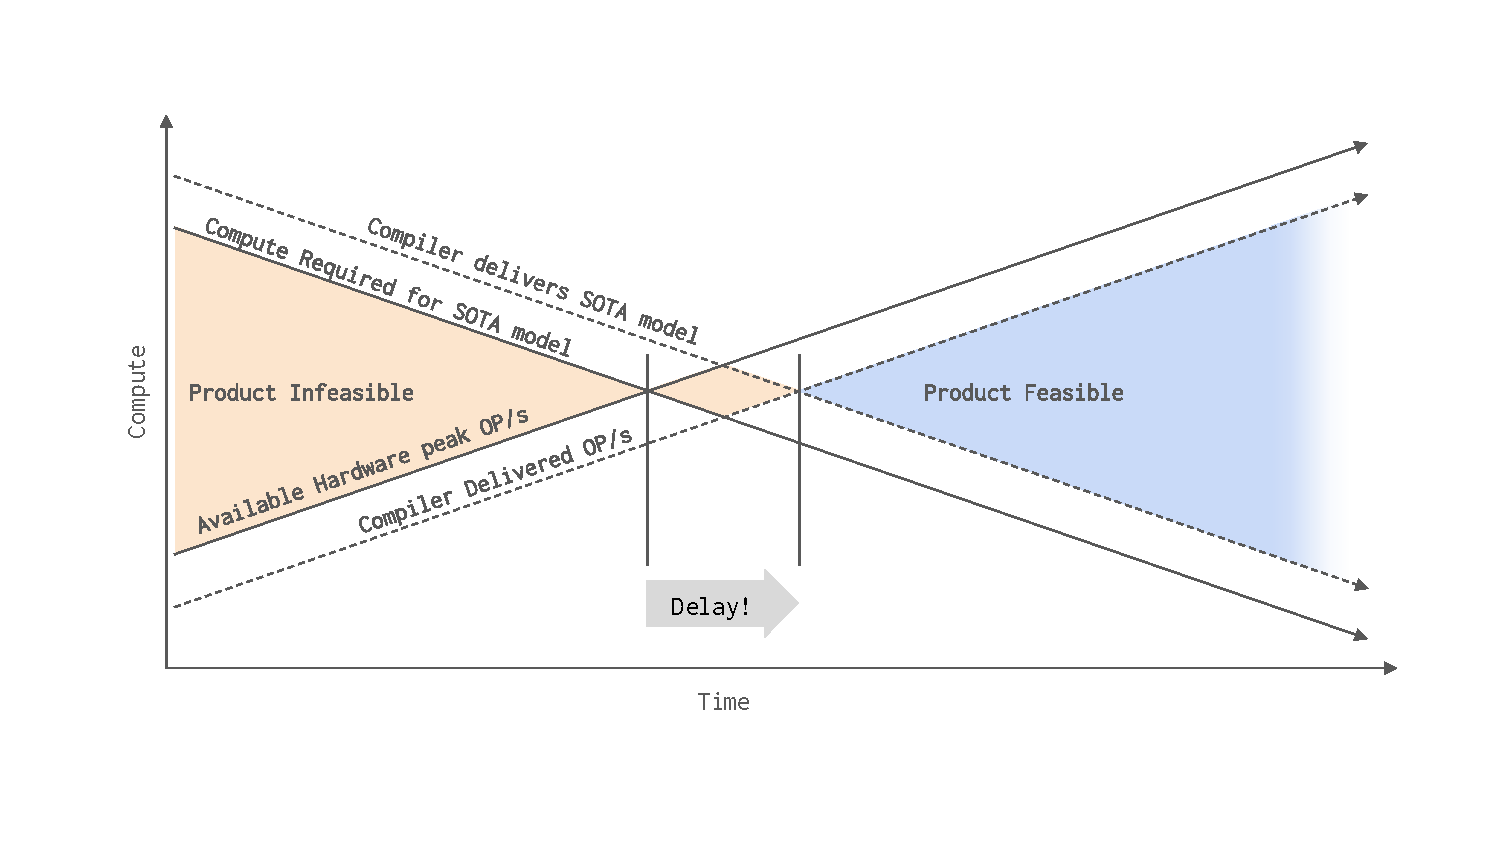
\includegraphics[width=\textwidth]{images/background/compilers_lagging.pdf}
    \caption{Compilers are lagging behind the development of both machine learning hardware and workloads. Figure created by Anton Lydike based on a slide from Sean Silva's talk at the March 2025 Cambridge Compiler Social.}
    \label{fig:compilers-lagging}
\end{figure}


\section{The LLVM compiler infrastructure}
\label{sec:llvm}

% SSA
% Peephole optimisation


% \subsection{User-extensible compiler infrastructure}
% To some degree LLVM cna be extended with intrinsics, but want to be able to define out own abstractions and stuff -> segues into MLIR


\section{MLIR}
\label{sec:mlir}

\subsection{IRDL}
\label{ssec:irdl}

\subsection{Pattern rewriting optimisations}
\label{ssec:pattern-rewriting}



\section{xDSL}
\label{sec:xdsl}









\section{Python internals}
\label{sec:python-internals}

% A brief overview of how Python works, talking about bytecode and stuff









\section{Static and dynamic languages}
\label{sec:static-dynamic-languages}

%% Define dynamism and dynamic/static languages
% Hook
Programming language design is a game of trade-offs, with a wide variety of design choices incurring differing benefits and costs, each of which impact a languages' suitability for a given task.
% Argument
One such choice is the degree of dynamism, defined by Williams et al. as ``allowing properties of programs to be defined at run-time'' \cite{williamsDynamicInterpretationDynamic2010}. As such, static languages fix properties ahead of time, whereas dynamic languages offer more flexibility at runtime.
% Link

%% Introduce mechanisms of dynamically/statically typed languages
% Hook
One common mechanism providing dynamism in programming languages is dynamic typing. This refers to programming languages where type-checking is performed at runtime, and variables can change type during the course of execution.
% Argument
In their essay ``The next 7000 programming languages'' \cite{chatleyNext7000Programming2019}, Chatley et al. discuss how the landscape of programming languages has changed since Landin's seminal 1966 paper ``The next 700 programming languages'' \cite{landinNext700Programming1966}. At the time of Landin's paper, there was already a split between dynamically typed languages such as Lisp and statically languages such as C and Algol. Lisp's runtime type checks incurred performance overhead and unexpected runtime type errors, but provided much greater expressivity and hence more productive development than static languages of the time. These trade-offs between static and dynamic languages remain much the same today, with Chatley et al. arguing that dynamically typed languages' expressivity results in ``excellent library support'', as they are better equipped to express structured data without a fixed schema.
% Link

%% Introduce other mechanisms of dynamism
% Hook
Beyond dynamic typing, there are a wide variety of other mechanisms by which programming languages can provide dynamism.
% Argument
One mechanism is runtime meta-programming, which refers to code which can introspect and manipulate its own behaviour at runtime. An example of this is monkey-patching in Python, which allows the programmatic modification of objects at runtime.
Another mechanism is late binding, which refers to resolving method calls at runtime when they are invoked, as opposed to being statically linked ahead of time. Interestingly, ahead-of-time compiled languages typically considered static such as C++ provide this dynamic behaviour in the case of polymorphism. When a method is invoked on an object in an inheritance hierarchy, the correct implementation to execute is resolved at runtime using C++'s vtable mechanism.
% Link
These dynamic aspects of languages influence the details of their implementation, and the degree to which they can be optimised.

%% Disentangling static/ahead-of-time compiled and interpreted/dynamic
% Hook
% Argument
% Link

%% Optimisation opportunities in dynamic and static languages
% Hook
Ahead-of-time compilers rely on static mechanisms such as data-flow analysis find valid optimisations.
% Argument
As they are run ahead of time, these static analyses have less information to reason about the dynamic runtime behaviour. In this dynamic case, some traditional optimisations cannot be guaranteed to be correct, and hence cannot be leveraged to improve program performance. For example, a function which is dynamically dispatched at runtime cannot be optimised through the code motion optimisation of function inlining, as the implementation which will be invoked is not known ahead of time.
Earlier work aims to address this, for example H\"olze and Ungar's paper ``Optimizing dynamically-dispatched calls with run-time type feedback'' \cite{holzleOptimizingDynamicallydispatchedCalls1994}. The authors provide an experimental compiler implementing ``type feedback'', a profile-guided optimisation which inlines dynamically dispatched calls in object-orientated languages.
However, such approaches are specific to individual aspects of the language runtime, and being ahead of time can only optimise for a prediction of the runtime behaviour.
% Link
Furthermore, runtime behaviour may differ significantly across inputs for some workloads, making this prediction less representative of real-world behaviour.

%% Dynamism of workloads
% Hook
In addition to considering support for dynamism as a property of a programming language, it can be helpful to classify a workload as dynamic or static.
% Argument
For example, \ac{gemm} operations which underpin modern machine learning systems rely on streaming data in a statically known order. This is well-suited to ahead-of-time compilation, as it is amenable to optimisation passes requiring no runtime information, such as code motion or vectorisation.
% TODO: Should this take my research domain as an example, or pick something else dynamic and can introduce my domain outside related work?
In contrast, pattern rewriting in user-extensible compiler frameworks relies on pointer chasing data structures with a high degree of dynamism. This is because the \ac{ssa} representation of the code being rewritten is structured as a doubly linked list, with the applications of the rewriting semantics to this list known only dynamically at runtime.
This dynamic, pointer-chasing workload incurs overhead and precludes many optimisations leveraged by ahead-of-time statically compiled languages such as C++ to accelerate their performance for other workloads.
% Link
% One crux of our research is extending the academic basis surrounding static and dynamic languages to quantitatively examine the difference in their performance for highly dynamic workloads.





% Object orientated optimisations (virtual dispatch in C++/objective-C)
% Why is JS faster than Python - more constrained

% Cranelift and arrays instead of linked lists for pattern rewriting (https://cfallin.org/blog/2020/09/18/cranelift-isel-1/)





















\section{JIT compilation}
\label{sec:jit-compilation}

% Hook
In their paper ``A Brief History of Just-In-Time'', Aycock defines \acf{jit} compilation as ``translation that occurs after a program begins execution'' \cite{aycockBriefHistoryJustintime2003}.
% Argument
He goes on to argue that \ac{jit} compilation approaches aim to accrue the benefits of both ahead-of-time compilation and interpretation, combining the runtime performance traditionally associated with compilation with the portability and access to runtime information of interpretation.
% Link

\subsection{JIT compilation to machine code}
\label{ssec:jit-compilation-machine-code}

% Hook
Whilst \acf{jit} compilation can refer to any program translation occurring at runtime, it is often overloaded to specifically refer to the dynamic generation of machine code.
% Argument
% Link

% V8 or something?

% \subsubsection{PyPy}
% \label{sssec:pypy}

% Hook
% Argument
% Link

% \subsubsection{Numba, JAX, and PyTorch}
% \label{sssec:numba-jax-pytorch}

% Hook
% Argument
% Link

\subsubsection{Copy-and-patch compilation}
\label{sssec:copy-and-patch-compilation}

%% Motivation
% Hook
\ac{jit} compilers
% A major bottleneck for traditional \ac{jit} compilation to machine code is the slow runtimes of optimising compilers.
% Argument
% Link
In their paper ``Copy-and-Patch Compilation'', Kjolstad and Xu present a novel approach to avoid this runtime cost.

%% Discuss
% Hook
Copy-and-patch compilation uses binary
% Argument
% Link

% Figure

% \subsubsection{Lua JIT}
% \label{sssec:lua-jit}

% Hook
% Argument
% Link



\subsection{Adaptive optimisation}
\label{ssec:adaptive-optimisation}

%% General case of using runtime information to change behaviour
% Hook
In addition to generating machine code on-the-fly, runtime information can be used to adapt program execution to the current workload.
% Argument
% Link

%% Motivation/intuition for the optimisation
% Hook
A significant overhead in the performance of dynamically typed languages is checking types at runtime, which is required to select the matching operation implementation for the type.
% Argument
Whilst this type information cannot be known ahead of time in dynamically typed languages, information collected at runtime can be used to optimised the type-checking process. This adaptive optimisation approach relies on the assumption that if a variable has had a fixed type for a sufficient span of time previously, it is likely that it will have the same type in future. For example, whilst a variable being used as an integer counter in a loop can take any value, if its type in the earlier iterations has always been an integer, it is likely to remain an integer throughout later iterations.
% Link
In an interpreted language, this assumption can be leveraged to replace general instructions with faster, specialised variants. A concrete implementation of this is Python's specialising adaptive interpreter, discussed in \autoref{sec:specialising-adaptive-interpreter}.
